\documentclass[14pt]{extarticle}
\def\activityid{F10-K-v2}\usepackage[letterpaper,margin=.65in,top=.60in,bottom=.65in]{geometry}
\usepackage[T1]{fontenc}
\usepackage[default]{sourcesanspro}
\usepackage{microtype,tikz,array,tabularx,fancyhdr,amsmath,amssymb}
\usepackage[hidelinks]{hyperref}
\usetikzlibrary{calc,arrows.meta}
\setlength{\parindent}{0pt}\setlength{\parskip}{7pt}
\setlength{\headheight}{0pt}\setlength{\footskip}{26pt}\setlength{\emergencystretch}{2em}
\pagestyle{fancy}\fancyhf{}\renewcommand{\headrulewidth}{0pt}\renewcommand{\footrulewidth}{.4pt}
\fancyfoot[L]{\scriptsize Bellingham Math Circle / Week 10 / \activityid}
\fancyfoot[R]{\scriptsize \thepage}
\definecolor{ink}{gray}{.12}\definecolor{soft}{gray}{.95}\color{ink}
\newcommand{\PageTitle}[2]{{\fontsize{10}{12}\selectfont\bfseries WEEK 10\quad ROUTE LAB\hfill #1\par}\vspace{3pt}{\fontsize{26}{29}\selectfont\bfseries #2\par}\vspace{2pt}}
\newcommand{\NameLine}{{\small Name: \rule{2.65in}{.4pt}\hfill Date: \rule{1.35in}{.4pt}\par}\vspace{4pt}}
\newcommand{\Task}[2]{\par\vspace{3pt}{\large\bfseries #1}\par #2\par}
\newcommand{\Subhead}[1]{\par\vspace{3pt}{\large\bfseries #1}\par}
\newcommand{\RuleBox}[1]{\par\begingroup\setlength{\fboxsep}{8pt}\colorbox{soft}{\parbox{\dimexpr\linewidth-16pt\relax}{#1}}\endgroup\par}
\newcommand{\WriteBox}[2]{\par\textbf{#1}\par\vspace{2pt}\begin{tikzpicture}\draw[black!40,line width=.5pt] (0,0) rectangle (\dimexpr\linewidth-.5pt\relax,#2);\end{tikzpicture}\par}
\newcommand{\StudentFooter}{\vfill{\small Try it with objects. Explain by pointing, talking, or drawing.}\par}
\newcommand{\RookBoard}[3]{\begin{tikzpicture}[x=#3,y=#3]\draw[step=1,black!45] (0,0) grid (#1,#2);\draw[thick] (0,0) rectangle (#1,#2);\node[font=\Large] at ({#1-.5},.5){$\star$};\draw[-{Latex},thick] (0,-.35)--(#1,-.35);\draw[-{Latex},thick] ({#1+.35},#2)--({#1+.35},0);\end{tikzpicture}}
\newcommand{\Table}[3]{\begin{tikzpicture}[x=#3,y=#3]\draw[step=1,black!25] (0,0) grid (#1,#2);\draw[thick] (0,0) rectangle (#1,#2);\fill (0,0)circle(3pt);\draw[-{Latex},very thick] (0,0)--(.7,.7);\node[below] at ({#1/2},-.1){width #1};\node[rotate=90,above] at (-.2,{#2/2}){height #2};\end{tikzpicture}}
\newcommand{\GraphNodes}{\coordinate(A)at(0,0);\coordinate(B)at(3,0);\coordinate(C)at(1.5,2.6);\coordinate(D)at(1.5,.95);}
\newcommand{\Kfour}[1]{\begin{tikzpicture}[scale=#1]\GraphNodes\draw[very thick](A)--(B)--(C)--(A)--(D)--(B) (D)--(C);\foreach \n in {A,B,C,D}{\node[circle,draw,fill=white,minimum size=22pt,font=\bfseries]at(\n){\n};}\end{tikzpicture}}
\newcommand{\House}[1]{\begin{tikzpicture}[scale=#1]\coordinate(A)at(0,0);\coordinate(B)at(3,0);\coordinate(C)at(3,2);\coordinate(D)at(0,2);\coordinate(E)at(1.5,3.3);\draw[very thick](A)--(B)--(C)--(D)--(A) (D)--(E)--(C);\foreach \n in {A,B,C,D,E}{\node[circle,draw,fill=white,minimum size=22pt,font=\bfseries]at(\n){\n};}\end{tikzpicture}}

\begin{document}

\PageTitle{K--1}{Cross every bridge once}\NameLine
\RuleBox{Dots are islands. Lines are bridges. Start on any island. Walk along every bridge \textbf{once}, without jumping. You may visit an island again. Put a counter on each bridge after using it.}
\Task{1. Explore the island town.}{Try a walk. Can you use every bridge and return to your starting island?}
\begin{center}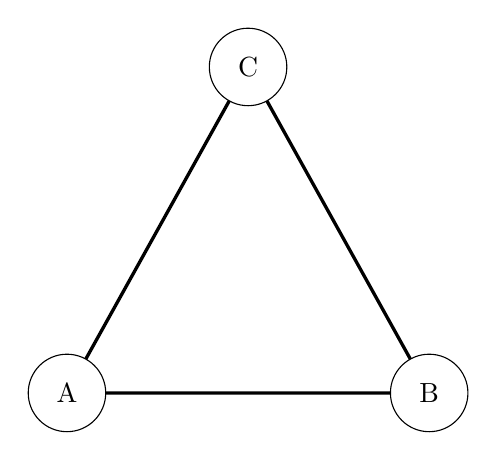
\begin{tikzpicture}[scale=2.3]\draw[very thick](0,0)--(2,0)--(1,1.8)--cycle;\foreach\p/\n in{0/A,1/B,2/C}{}\node[circle,draw,fill=white,minimum size=28pt]at(0,0){A};\node[circle,draw,fill=white,minimum size=28pt]at(2,0){B};\node[circle,draw,fill=white,minimum size=28pt]at(1,1.8){C};\end{tikzpicture}\end{center}
\Task{2. Add a little branch.}{An adult draws one new bridge from A to a new island D. Can you still use every bridge once? Where can you start? Where must you finish?}
\WriteBox{Show your new map or tell an adult your route.}{1.25in}
\StudentFooter

\newpage

\PageTitle{K--1}{Why do dead ends matter?}\NameLine
\Task{3. Try this town.}{Can one walk use every bridge once? Try more than one starting island.}
\begin{center}\begin{tikzpicture}[scale=1.8]\draw[very thick](0,0)--(0,2) (0,0)--(-1.6,-1) (0,0)--(1.6,-1);\foreach\n/\x/\y in{A/0/0,B/0/2,C/-1.6/-1,D/1.6/-1}{\node[circle,draw,fill=white,minimum size=28pt]at(\x,\y){\n};}\end{tikzpicture}\end{center}
\textbf{Think with your finger:} If you visit a leaf island in the middle of a walk, how can you leave without reusing its bridge?
\Task{4. Repair it.}{Add \textbf{one} bridge between two leaf islands. Try your walk again. Did you need to start somewhere special?}
\WriteBox{Draw your repair and show a complete route.}{1.20in}
\StudentFooter

\end{document}
